\section{Creating a Language Model for German}\label{lm}

The learning curve above was plotted using the results from training on English samples. To compare get an intuition about whether the conclusions made are transferable to training on samples in other languages, the training was done again on German samples. In order to do this, a \ac{LM} for German had to be created first. 

\subsection{n-Gram Language Models}

To understand the following sections better it might be helpful to get a quick recap about \ac{LM}. \ac{LM} are probabilistic models that model the likelyhood of a given sequence of characters or words. The most widely used type for word-based models \ac{LM}s are $n$-gram \ac{LM}. However, such models can estimate probabilities only for words that appear in the vocabulary of the corpus they were trained on. All other words are \ac{OOV} words with a probability of $0$. Single words are $1$-grams, but the same applies for $n$-grams of any order. But because of combinatorial explosion the $n$-gram, such \ac{LM} suffer from sparsity with increasing order $n$. To handle \ac{OOV} issues efficiently, a technique called \textit{smoothing} is applied. A very rudimentary form of smoothing is \textit{Laplace Smoothing}, which assigns a minimal count of $1$ to every $n$-gram. All other counts are also increased by adding $1$. This prevents counts of zero, which is important when calculating the perlexity of a model (because the count appears in the divisor and we cannot divide by zero) Although with Laplace Smoothing a very low probability is assigned to previously unseen $n$-grams (which results in a high perplexity), it performs poorly in application. A better way of smoothing is achieved using \textit{Kneser-Ney Smoothing}.

\subsection{Creating a raw text corpus and training the model}

A LM was trained on a raw text corpus of German Wikipedia articles using KenLM \parencite{kenlm}. The articles were pre-processed to meet the requirements of \textit{KenLM}.
It was normalized by removing Wiki markup, punctuation and making everything lowercase. Accentuated characters (like \code{è,é,ê}, etc.) and special characters like the German \textit{ß} were translated to their most similar ASCII-equivalent (\code{e} resp. \code{ss}) to account for ambiguous spelling and reduce the number of words. Umlauts (although not part of the ASCII codeset) were kept as-is because they are used very frequently in German. 

Because \textit{KenLM} expects the input as sentences (one sentence per line), the raw text was further tokenized into sentences and words using NLTK \parencite{nltk}. Word tokens that contain only numeric characters (such as year numbers) are changed to \code{<unk>}, a special token which is traditionally used to denote an \ac{OOV} word. Although numeric tokens occur frequently in the Wikipedia articles, they are unwanted in the corpus because they do not carry any semantic meaning and because there is an infinite number of possible numbers.

The following lines are an excerpt of a article in the German Wikipedia along with its representation in the corpus.

\begin{displayquote}[German Wikipedia article about Speech Recognition\footnote{\url{https://de.wikipedia.org/wiki/Spracherkennung}}]
Die Größe des Wörterbuchs hängt stark von der Sprache ab. Zum einen haben durchschnittliche deutschsprachige Sprecher mit circa 4000 Wörtern einen deutlich größeren Wortschatz als englischsprachige mit rund 800 Wörtern. Außerdem ergeben sich durch die Flexion in der deutschen Sprache in etwa zehnmal so viele Wortformen, wie in der englischen Sprache, wo nur viermal so viele Wortformen entstehen.
\end{displayquote}

\begin{lstlisting}[numbers=left, caption=Representation in corpus]
die grösse des wörterbuchs hängt stark von der sprache ab
zum einen haben durchschnittliche deutschsprachige sprecher mit circa <unk> wörtern einen deutlich grösseren wortschatz als englischsprachige mit rund <unk> wörtern
ausserdem ergeben sich durch die flexion in der deutschen sprache in etwa zehnmal so viele wortformen wie in der englischen sprache wo nur viermal so viele wortformen entstehen
\end{lstlisting}

The final corpus contained data from 2,221,101 Wikipedia articles (42,229,452 sentences, 712,167,726 words, 8,341,157 unique words). A $4$-gram \textit{KenLM} model was trained on this corpus. KenLM uses \textit{Kneser-Ney Smoothing} and automatically adds the unigrams \code{<s>, </s>} and \code{<unk>} internally for sentence beginnings, endings and \ac{OOV} words). $n$-grams can be represented with a tree structure \footnote{note that \textit{KenLM} offers a so called \textit{PROBING} data structure, which is fundamentally a hash table combined with interpolation search, a more sophisticated variant of binary search, which allows for constant space complexity and linear time complexity. This does however not change the fact that $n$-grams can conceptually be thought as a tree of grams}, which allows for pruning. Pruning 1-grams would help getting rid of obvious spelling mistakes and very rare tokens that only appear in very special contexts. Unfortunately, \textit{KenLM} does not support pruning unigrams, only higher-order $n$-grams. Therefore the vocabulary used for training was limited to the 500,000 most frequent words not containing numbers with a minimum length of 2 characters \footnote{this constraint was imposed because NLTK did sometimes not tokenize abbreviations like \textit{z.B.} correctly, which resulting in two separate tokens \code{z} and \code{b}}. This amount is about the same what was used in the \textit{DeepSpeech} paper \parencite{deepspeech}. The words in the vocabulary make up 96.42\% of the whole corpus. The most frequent word in the vocabulary is the \code{<num>} token (29,659,021 counts), the least frequent word is \textit{Flachmeeres} (31 counts). Note that the latter is actually a derivate of another German word \textit{Flachmeer}, which also appears in the vocabulary (109 counts). Having different flexions of the same word is characteristic for German texts. Handling them would require lemmatization and/or stemming the corpus, which has not been done for simplicity. It is also doubtful whether this would actually help improving the quality of inferred transcripts, since humans do not speak in lemmata or stems.

By limiting the vocabulary to the 500k most frequent words, the unigrams in the KenLM were artificially pruned. The number of unigrams was therefore 500,003 (one unigram for each word in the vocabulary plus one each for the \code{<s>}, \code{</s>} and \code{<unk>} tokens). The $n$-grams used to train the \ac{LM} have been pruned by setting the minimal threshold for $n$-Grams of any order ($n \in 1..4$) to 40. This is the value that Google used (reference from Jurafsky). Pruning unigrams helped getting rid of obvious spelling mistakes and very rare tokens that only appear in very special contexts (like the tokens \textit{aaaaa} or \textit{zzyzzyxx}) (EDIT: Pruning unigrams is not supported by KenLM, but the vocabulary can be limited). Such words are mostly not no real German words and should therefore not be trained on. Pruning higher-order $n$-grams was done to increase performance (both in space and time).

\subsection{Evaluating the model}

The best way to evaluate a \ac{LM}is to embed it in an application and measure how much the application improves \parencite{slp3}. This is called \textit{extrinsic evaluation} and has been done by comparing the learning curves with and without using a \ac{LM}. However, to measure the performance of a \ac{LM} independently (\textit{intrinsic evaluation}) one would have to provide a test set containing unseen sentences an assess the scores of the \ac{LM} on their $n$-grams. The results can then be compared to a reference \ac{LM}: Whatever model produces higher probabilities (or lower perplexity) to the $n$-grams in the test set is deemed to perform better. However, because models can only be compared if they use the same vocabulary \parencite{slp3}, this would require training the reference model would need to be trained on the same corpus, which can become very time consuming.

\textit{KenLM} has been extensively compared to other \ac{LM} implementations like \ac{SRILM} both in terms of speed and accuracy. It has been found to be both faster and more memory efficient \parencite{kenlm} than the fastest alternative. Its low memory profile makes it runnable on a single machine, while other algorithms like \textit{MapReduce} target clusters \parencite{kenlm_estimation}. This was a big advantage especially for this project. The probabilistic performance of \textit{KenLM} has been evaluated by training a $5$-gram model on a 126 billion token corpus (393 unique words) \parencite{kenlm_estimation}. This model was embedded in some Machine Translation systems (Czech-English, French-English and Spanish-English) . Evaluation was done by calculating the BLEU score and comparing it to embeddings of other \ac{LM}. \textit{KenLM} placed first in all submissions.

Because of time constraints and because \textit{KenLM} has already been extensively evaluated on English I resign from evaluating my German \ac{LM} intrinsically, although the corpus used for training is not as big as the one used in \cite{kenlm_estimation}. To this day \textit{KenLM} is widely recognized as the best performing \ac{LM} out there, which is also emphasized by the usage of a \textit{KenLM} model in the Mozilla implementation of \textit{DeepSpeech}.

To still get an intuition about how well the model performs, two different experiments were made:

\begin{itemize}
	\item \textbf{Experiment 1}: The probability calculated for valid German sentences was compared against variants of the same sentences where the words appear in randomized order.
	\item \textbf{Experiment 2}: The \ac{LM} was used together with its vocabulary to build a simple word predictor.
\end{itemize}

Both experiments are explained in more depth below.

\subsubsection{Evaluation 1: Comparing scores of randomized sentences}

The first experiment tests the validity of the probabilities (\textit{scores}) calculated by the \ac{LM}. For this, an arbitrary choice of 5 valid sentences in German was used. To make sure the sentences could not have been seen during training, the following 5 sentences were taken out of the current newspaper (dated after the creation of the Wikipedia dump):

\begin{itemize}
	\item \textit{Seine Pressebeauftragte ist ratlos.}
	\item \textit{Fünf Minuten später steht er im Eingang des Kulturcafés an der Zürcher Europaallee.}
	\item \textit{Den Leuten wird bewusst, dass das System des Neoliberalismus nicht länger tragfähig ist.}
	\item \textit{Doch daneben gibt es die beeindruckende Zahl von 30'000 Bienenarten, die man unter dem Begriff «Wildbienen» zusammenfasst.}
	\item \textit{Bereits 1964 plante die US-Airline Pan American touristische Weltraumflüge für das Jahr 2000.}
\end{itemize}

For each of these sentences the score was calculated. Then the words of the sentences were shuffled and the score was calculated again. A good \ac{LM} should calculate a (much) higher probability for the original sentence, because the shuffled sentence is most likely to be gibberish. All sentences have been normalized the same way sentences were preprocessed for training. Table \ref{LM_evaluation} shows the results of the comparison. It is evident that the probabilities for the shuffled sentences are much lower than for the sentences where the words appear in the correct order. The probabilities calculated by the \ac{LM} are therefore deemed valid.

\begin{table}[!htbp]
	\centering
	\begin{tabular}{|l|r|l|r|}
		\hline
		\thead{original sentence (normalized)} & \thead{score} & \thead{permuation} & \thead{score} \\
		\hline
		\makecell[l]{seine pressebeauftragte\\ist ratlos} & -17.58 & \makecell[l]{ist ratlos\\pressebeauftragte seine} & -21.52 \\ 
		\hline
		\makecell[l]{fünf minuten später steht\\er im eingang des kulturcafes\\an der zürcher europaallee} & -40.23 & \makecell[l]{des er minuten zürcher kulturcafes\\steht europaallee eingang\\fünf im später an der} & -57.69 \\ 
		\hline
		\makecell[l]{den leuten wird bewusst\\dass das system des \\ neoliberalismus nicht\\länger tragfähig ist} & -35.52 & \makecell[l]{system nicht das ist\\dass leuten tragfähig des\\neoliberalismus den\\bewusst länger wird} & -51.27 \\
		\hline
		\makecell[l]{doch daneben gibt es die\\beeindruckende zahl von \code{<num>}\\bienenarten die man unter dem\\begriff wildbienen zusammenfasst} & -48.36 & \makecell[l]{dem gibt wildbienen zahl\\beeindruckende doch man\\zusammenfasst es daneben bienenarten\\von die unter die \code{<num>} begriff} & -75.95 \\
		\hline		
		\makecell[l]{bereits \code{<num>} plante\\die usairline pan american\\touristische weltraumflüge\\für das jahr \code{<num>}} & -58.04 & \makecell[l]{plante touristische für\\jahr pan american das\\bereits usairline \code{<num>}\\\code{<num>} weltraumflüge die} & -64.02 \\
		\hline		
	\end{tabular}
	\caption{Comparison of log10-probabilities calculated for news sentences and a permutation of their words}
	\label{LM_evaluation}
\end{table}

\subsubsection{Experiment 2: Word predictor}

The second experiment tests whether the trained \ac{LM} is able to continue a sentence given its beginning. For this each word from the vocabulary is appended and the score of the resulting stumps is calculated. The most likely continuation can be estimated by sorting the resulting list in descending order (the probabilities are $\log_10$-based, i.e. negative) and taking the first element. This behavior can be applied iteratively to construct a sentence from a stump. For this experiment a sentence was started with the stump \textit{Ein - 2007 - erschienenes}. Afterwards a word from the five most probable continuations was appended. The extended stump was then again fed into the \ac{LM}. This process was repeated until some kind of sentence ending was encountered. Eacg extended stump was preprocessed the same way the sentences were preprocessed for training (lowercasing, replacing numbers with \code{<num>}, etc.). Figure \ref{word_predictor} shows the path taken through the predictions. Note that the predictions for the second and third word of the stump after typing the first word are shown in grey for illustrative purposes, although they were not considered for continuation.

\begin{figure}
	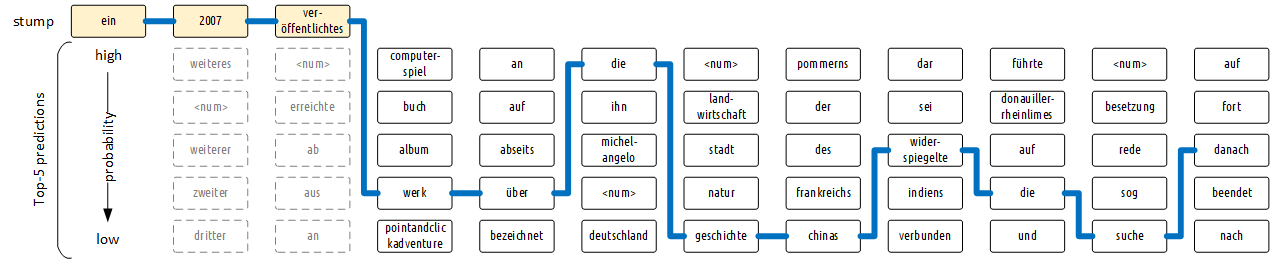
\includegraphics[width=\linewidth]{./img/word_predictor.png}
	\caption{Word predictions of the trained 5-gram model for continuations of the stump \textit{«Ein 2007 erschienenes ...»}. The blue path represents a grammatically valid German sentence.}
	\label{word_predictor}
\end{figure}

Although prediction was slow we can observe that the words suggested by the \ac{LM} are generally grammatically correct continuations and often make sense, although the probability for some of the predicted words (like \textit{Michelangelo}) is sometimes unexplicably high. Nevertheless it was possible to create a grammatically correct German sentence from the stump using only the suggested words. The \ac{LM} even seems to have captured some notion about grammatical concepts like German cases (e.g. that \textit{"die Geschichte Chinas"} is more likely than \textit{"die Geschichte China"}). On the other hand we can observe that the meaningfulness of the suggestions decreases with the progress because some long-distance relationships between words are lost for small values of $n$.

%score for 'ein': -2.5511488914489746
%top 5 words:
%word        log10-probability
%--------  -------------------
%weiteres             -5.973
%<num>                -6.00614
%weiterer             -6.18446
%zweiter              -6.21412
%dritter              -6.30031
%
%score for 'ein <num>': -4.864611625671387
%top 5 words:
%word         log10-probability
%---------  -------------------
%<num>                 -7.34603
%erreichte             -7.75604
%ab                    -7.77345
%aus                   -7.86214
%an                    -7.87674
%
%score for 'ein <num> erschienenes': -7.372537136077881
%top 5 words:
%word                      log10-probability
%----------------------  -------------------
%computerspiel                      -8.47756
%buch                               -8.86841
%album                              -9.2071
%werk                               -9.30259
%pointandclickadventure             -9.31129
%
%score for 'ein <num> erschienenes werk': -8.43615436553955
%top 5 words:
%word          log10-probability
%----------  -------------------
%an                     -10.5713
%auf                    -10.863
%abseits                -10.9379
%über                   -11.0053
%bezeichnet             -11.0132
%
%score for 'ein <num> erschienenes werk über': -9.723254203796387
%top 5 words:
%word            log10-probability
%------------  -------------------
%die                      -12.0887
%ihn                      -12.1763
%michelangelo             -12.4766
%<num>                    -12.4973
%deutschland              -12.5661
%
%score for 'ein <num> erschienenes werk über die': -9.965542793273926
%top 5 words:
%word              log10-probability
%--------------  -------------------
%<num>                      -11.9341
%landwirtschaft             -12.1469
%stadt                      -12.2681
%natur                      -12.2898
%geschichte                 -12.5322
%
%score for 'ein <num> erschienenes werk über die geschichte': -11.084966659545898
%top 5 words:
%word           log10-probability
%-----------  -------------------
%pommerns                -12.7682
%der                     -13.4756
%des                     -13.5903
%frankreichs             -13.6889
%chinas                  -13.7065
%
%score for 'ein <num> erschienenes werk über die geschichte chinas': -13.830591201782227
%top 5 words:
%word              log10-probability
%--------------  -------------------
%dar                        -14.8973
%sei                        -14.9483
%widerspiegelte             -15.1113
%indiens                    -15.555
%verbunden                  -15.6136
%
%score for 'ein <num> erschienenes werk über die geschichte chinas widerspiegelte': -15.959598541259766
%top 5 words:
%word                    log10-probability
%--------------------  -------------------
%führte                           -19.0873
%donauillerrheinlimes             -19.3014
%auf                              -19.3185
%die                              -19.3199
%und                              -19.3243
%
%score for 'ein <num> erschienenes werk über die geschichte chinas widerspiegelte die': -17.793916702270508
%top 5 words:
%word         log10-probability
%---------  -------------------
%<num>                 -19.5746
%besetzung             -20.353
%rede                  -20.706
%sog                   -20.7197
%suche                 -20.7211
%
%score for 'ein <num> erschienenes werk über die geschichte chinas widerspiegelte die suche': -19.95460319519043
%top 5 words:
%word       log10-probability
%-------  -------------------
%auf                 -21.5493
%fort                -21.8571
%danach              -21.8975
%beendet             -22.052
%nach                -22.0672

%score for 'ein <num> erschienenes werk über die geschichte chinas widerspiegelte die suche danach': -22.0571231842041
%top 5 words:
%word           log10-probability
%-----------  -------------------
%diskutiert              -23.6575
%abzielen                -23.9694
%begeben                 -23.9833
%beeinflusst             -24.0387
%auf                     -24.0435